Each of the required read and write functions of the assignment were implemented.
The novel functionality was also implemented. Documentation was created
using ``Doxygen'' and can be found in the submit git repository.

Figures \ref{fig:images-git1} and \ref{fig:images-git2} show the GitLab commit
history for the assignment. This does not demonstrate the full history of the
project, as a number of merged branches were later deleted, however all major
changes are reflected in the screenshots.

\begin{figure}[H]
	\centering
	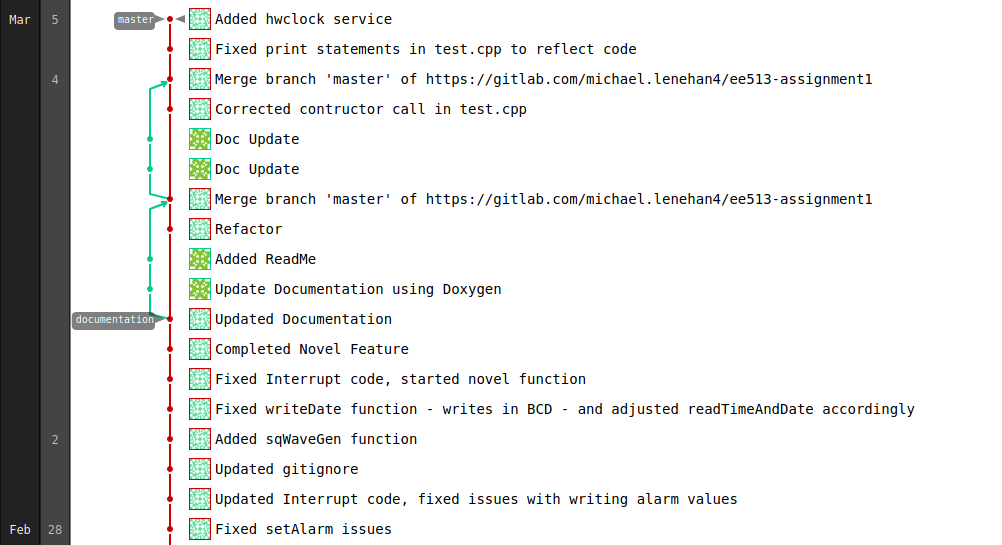
\includegraphics[width=0.8\textwidth]{images/git1}
	\caption{GitLab Commit History}
	\label{fig:images-git1}
\end{figure}

\begin{figure}[H]
	\centering
	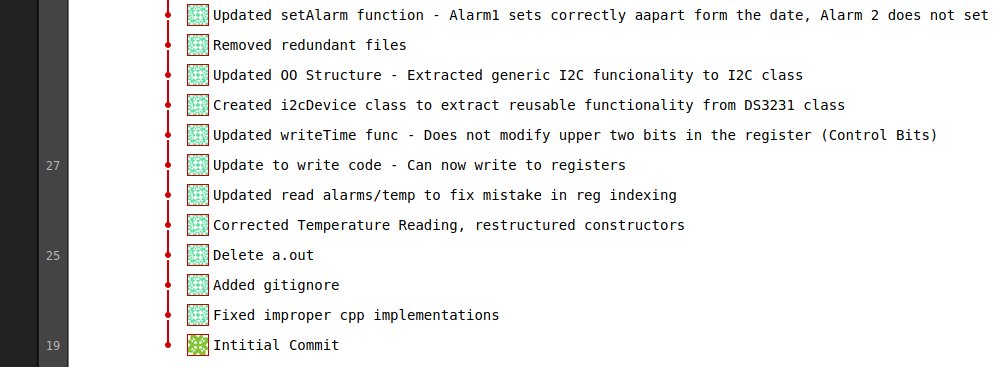
\includegraphics[width=0.8\textwidth]{images/git2}
	\caption{GitLab Commit History}
	\label{fig:images-git2}
\end{figure}

The interrupt
did not operate as expected. Reading the datasheet indicates that the interrupt
bit being set high while the alarm flag is low would result in no output on the
square wave output, however the exact opposite is true, with no output on the
pin only if the alarm flag is high.

Overall a lot was learned with regards to integrating hardware with an embedded
Linux system, including how to communicate via I2C, and how to perform
integration testing.
